
The aim of this paper is to serve as a manual for using the software application
given. With the aid of this manual, the reader should be prepared for solving
initial condition problems using high-order finite-difference schemes.\\

A whole and precise description of the subroutines and procedures joined under
the program structure is beyond the bounds of this work. The purpose of this text is
to familiarise the reader with the numerical approach to these problems and to
give the essential information in order to use the software.  \\

The most part of the effort will be dedicated to the description of the
\underline{application programming interface} of this software. An API is an
ensemble of procedures and subroutines which determines how a piece of the program interacts
with an other.  \\

After the read of this paper the user will understand the first
layer of the program, and will be able to write his/her problems
according to the API's structure. 



%1.==========================BODY==============================================
\newpage

\section{Introduction}

An initial-boundary value problem is one of the most generic structures in
mathematics. It can involve both temporal and spatial derivatives. Generally
speaking, we may find something in the shape of: 

\begin{Large}
$$\begin{cases} \frac{d \mathbf{U}}{dt}=   {\mathscr{L}}( \mathbf U,
	t, \mathbf x) \\[0.25cm]
	\hspace {0.25cm}+ IC \quad + BC
	\end{cases}$$
\end{Large}
\\

Where the $\mathscr{L}$ includes any mathematical operator, so the problem can
be an ordinary differential equation (\textit{ODE}) and also a partial
differential equation (\textit{PDE}). \\

The method for the numerical resolution of this problem involves the
transformation of the problem to an easier structure. \\

First of all the general problem should be reduced to an ODE. Usually, this step
involves the \underline{spatial discretization} of the problem. Once this
operations are finished, the equations should have the following structure: 


	$$\begin{cases} \frac{d \mathbf{U}}{dt}=  \mathbf F( \mathbf U, t)  \\[0.25cm]
	\hspace {0.25cm}+ IC 
	\end{cases}$$
	\\
	
This is known as \underline{Cauchy problem} in the mathematical bibliography.
There exist a huge collection of methods and procedures for solving problems
under this structure. The importance of this expression is that any
initial-boundary value problem can be reduced to this, so once the right part of
the assignment (the $\mathbf F( \mathbf U, t)$) is defined, the numerical
solution of the resulting equation implicates always the same steps. The idea of
the library is to hold the procedures so it can be launched for any given
problem.\\

The approach to the numerical solution of any given problem can be summarized in
the following chart: \\

\begin{framed}

\framebox[3cm]{\textbf{Physics}}% 
	\hfill
	\framebox[12cm]{\textbf{Mathematics}} \\
	
{\begin{small}	
	
\framebox[3cm]{$\begin{cases}\text{Equations}\\ 
+IC +BC\end{cases}$}%
$\: \Rightarrow  {\mathscr{L}}( \mathbf U,
	t, \mathbf x)\: \rightarrow$
\framebox[2.5cm]{$\begin{matrix} \text{Spatial}\\
\text{discretization}\end{matrix}$}%
$ \: \rightarrow \mathbf F( \mathbf U, t)\rightarrow$
\framebox[2.5cm]{$\begin{matrix} \text{Temporal}\\
\text{discretization}\end{matrix}$}
$\: \Longrightarrow \: \mathbf{U}(t)$

\end{small}}

\end{framed}

\vspace{1cm}

The idea of the software application is to hold the operations contined under
the label \textit{mathematics}. This way, the resolution of the problems will be
automatic, once the \textit{physics} are defined. \\

The advantage of proceding this way is that all the complex mathematical
operations are encapsulated inside the library \textbf{Cauchy\_Problem}, where
the routines and procedures have been carefully defined, tested and validated.
All the operations are structured in layers, and the effort of the user
is reduced to the definition of the higher one: the \underline{Application
Layer}, where the problem should be written according to the \textbf{API} of
the layers underneath.\\

The purpose of this manual is to help with the construction of the application layer, according to the specific rules and
procedures that the API fixes. \\

So, the software application has the following structure: \\

\begin{framed}

\begin{framed}
\centering 
{\Large \textbf{Application layer}}


\end{framed}

\begin{multicols}{2}
\centering
$\Uparrow \:API_{HOFD}\: \Downarrow$

\begin{framed}

\textbf{Spatial semi-discretization}

\begin{multicols}{2}
\begin{framed}
Grids\\
\end{framed}

\columnbreak

\begin{framed}
{{Finite\\ differences}}
\end{framed}

\end{multicols}

\begin{framed}
Lagrange interpolation
\end{framed}

\end{framed}

\centering
$\Uparrow \:\: \Downarrow$

\columnbreak 

\centering
$\Uparrow \:API_{Cauchy Problem}\: \Downarrow$

\begin{framed}
\textbf{Temporal semi-discretization}

\begin{framed}
Cauchy Problem
\end{framed}
\vspace{0.3cm}

\begin{framed}
Temporal schemes\\
\end{framed}

\end{framed}
\centering
$\Uparrow \:\: \Downarrow$


\end{multicols}

\begin{framed}
\centering Numerical recipes (linear/non linear algebra)
\end{framed}

\end{framed}

Where \underline{only the application layer} is to be changed, while all the
other modules are encapsulated inside the library. \\

%==================================

\newpage
\subsection{Examples of application}

In this section we are going to deal with three different problems in a higher
complexity scale. We will see how the problem can be transformed to something
in the shape of what he have been talking about.\\

 First of all, an ODEs problem is presented, the well-known
mass-spring-damper system. The advantage of this problem is that we will not
need the spatial discretization, since spatial derivatives are not included in
the problem's definition.\\

Then we will deal with Lorenz attractor. This is also an ODEs problem, this
time involving multiple dimensions.\\

Finally we will reach an intial value PDEs problem, whose numerical
resolution procedure involves all the actions we have described in this
section. \footnote{go to the appendices to check the software implementation
of these problems.}\\

\subsubsection*{Mass-spring-damper system}

The following problem is considered:
$$
M \ddot x + D \dot x + K x = P(t)
$$

With the initial conditions: 
$$
x(t=0)=x_0; \;\;\; \dot x (t=0)= \dot x_0
$$\\

First of all, the problem must be transformed into a first order derivative
(Cauchy problem structure).

For this purpose, a vector of unknown variables is defined:
$$
U=[x,  \dot x] \Longrightarrow \frac{d \mathbf{U}}{dt}= \mathbf{F}(\mathbf{U},t)
$$
$$
\frac{d}{dt}\begin{bmatrix}
U(1)\\
U(2)
\end{bmatrix}= 
\begin{bmatrix}
F(1)\\
F(2)
\end{bmatrix}
\Longrightarrow \mathbf{F}=\begin{bmatrix}
U(2)\\
\frac{1}{M}\cdot (P(t)-D\cdot U(2)-K \cdot U(1))
\end{bmatrix} 
$$\\

This function $F=F(U)$ is going to be named \underline{system} in the software
application.
As we can see, even in a simple example is a vector function.\\

Now that the Cauchy problem is defined, the program is able to continue with the
numerical resolution. Here, some opetions must be chosen (numerical scheme,
duration, time steps\ldots). For the shake of simplicity let's assume we want to
use an explicit Euler scheme:\\

\begin{framed}
$$
n=0,\;\; t=t_0, \;\; \mathbf{U}^0=[x_0, \dot x_0]
$$

\begin{framed}
$n \rightarrow$ \framebox[5cm]{$\mathbf{F}^n=\mathbf{F} (\mathbf{U}^{n})$}% 
	$\rightarrow$
	\framebox[5cm]{$\mathbf{U}^{n+1}=\mathbf{U}^n + \Delta t \cdot \mathbf{F}^n$}% 
	$\rightarrow$
	$\mathbf{U}^{n+1}$ \\
	$$\longleftarrow n=n+1 \longleftarrow$$
\end{framed}

\end{framed}

\subsubsection*{Lorenz attractor}

Now we are going to consider the following problem: 
{\large{
$$
\begin{cases}
\frac{dx}{dt}= a \cdot ( y - x ) \\
\frac{dy}{dt} =x \cdot ( b - z ) - y \\ 
\frac{dz}{dt} =x \cdot y - c \cdot z \\
\end{cases}
$$
}}
$$
x(t=0)=x_0;\;\; y(t=0)=y_0;\;\; y(t=0)=y_0
$$\\

As we can see, this is already a first order derivative problem. So, the
transformation is inmediate: 
$$
\mathbf{U}=[x,y,z] \longrightarrow \frac{d}{dt} \begin{bmatrix}
U(1)\\
U(2)\\
U(3)
\end{bmatrix}= 
\begin{bmatrix}
a \cdot ( U(2) - U(1) ) \\
U(1) \cdot ( b - U(3) ) - U(2) \\ 
U(1) \cdot U(2) - c \cdot U(3) \\
\end{bmatrix}=\begin{bmatrix}
F(1)\\
F(2)\\
F(3)
\end{bmatrix}
$$\\

The connection with the previous problem is evident, 
$$
\frac{d \mathbf{U}}{dt}= \mathbf{F}(\mathbf{U},t)
$$

Therefore, we can think of a first extrapolation: once we arrive to a
\textbf{Cauchy problem}, \underline{the solving procedure is the same}.\\

\newpage
If we assume we have a solver for this type of problems, the input arguments to
this program should be something like: \\

\begin{framed}
\textbf{Cauchy problem} \\

\hspace{1cm} Initial conditions ($\mathbf{U}^0$)

\hspace{1cm} System ($\mathbf{F}(\mathbf{U},t)$)

\hspace{1cm} Temporal scheme (Explicit Euler in the previous example)

\hspace{1cm} Time iteration ($n$)
\end{framed}

\vspace{1 cm}

With this structure both the previous (mass-spring-damper) and this program
(lorenz attractor) can be solved.\\

The importance of this structure is that the same piece of code will be useful
for solving a huge amount of problems, so a great deal of time and effort is
saved. Also, this method allows us to test the different modules separetely, in
order to assure its functionallity. Finally, but any less important, we can
change the resolution process (temporal scheme/time domain) with little effort.
This might be decisive when dealing with stability matters. \\

\newpage

Now, let's look how the Cauchy problem is written in the program: \\

\begin{blueframed}
{\small
\begin{lstlisting}
subroutine Cauchy_Problem_Solution( Domain,  Initial_C, System, 
				Scheme, Outputs) 
        
     procedure (Temporal_Domain)  :: Domain 
     procedure (Initial_Condition) :: Initial_C
     procedure (System_ODES) :: System
     procedure (Temporal_Scheme), optional :: Scheme
     procedure (ODES_Outputs), optional :: Outputs 
     
     ![...]
\end{lstlisting}
}
\end{blueframed}

\vspace{0.5cm}

We can see that this is pretty much the very same structure that the one shown
in the conceptual construction.\\

The subroutine needs the input arguments of time, system and initial conditions. The temporal
scheme is declared as optional: if there is not an specific choice, the program
will continue with the default procedure (Runge-Kutta RK4).
\\

The subroutine also includes another procedure which is used to extract
information from the resolution process (${ODES\_ Outputs}$), but it is
not necessary for the program to run (it has the label \textit{optional}).\\

Summarizing for fixing ideas: when dealing with problems, we are not
interested in developing a specific software for each equation. It is much
more efficient to generate a procedure which can be used equally for different
problems (\textit{interchangeability}).\\

With this two examples, we have seen how two different problems are solved with 
the same routine. Although the problems
were simple, the idea behind these examples is very powerful; and it will be
demonstrated with the next problem, which involves also spatial
discretization.\\

\subsubsection*{Heat equation 1D}

We are going to deal with the following problem:
$$
\rho \cdot c_p \frac{\delta u}{\delta t}= k \frac{\delta^2 u}{\delta x^2};\;\;\;
+IC; \;\;\; +BC
$$

The procedure for solving this equation can be divided in two groups of
operations as we have seen before: spatial semi-discretization and the
resulting Cauchy problem (as this problem is already a first-order derivative;
otherwise some other operations must be done).\\

\newpage
a) Spatial semi-discretization\\

\begin{figure}[h]
\centering
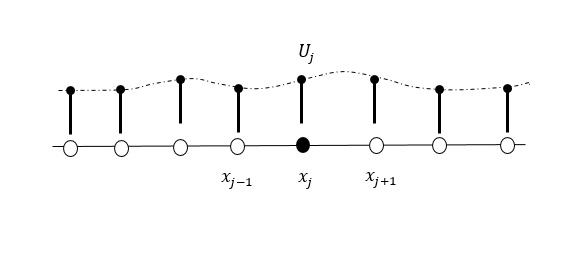
\includegraphics[scale=0.7, trim = 30mm 15mm 25mm 0mm,
clip]{./Figures/2-CauchyProblem/spatial_discretization.jpg}
\caption{Spatial discretization}
\end{figure}

$$
\frac{\delta u}{\delta t}= \frac{k}{\rho \cdot c_p } \frac{\delta^2 u}{\delta
x^2} \Longrightarrow \left(\frac{\delta^2 u}{\delta
x^2}\right)_{x=x_j} = f(U_{j-p},\ldots U_j \ldots U_{j+q})$$

$$
BC \Longrightarrow g(U_0,U_1,\ldots)=0;$$\\

For example, using equally-spaced second order interpolation, 
$$
x_j= a+(b-a) \cdot \frac{j}{m}; \;\;\; j\in [0,m]
$$
$$
\Delta x= x_j-x_{j-1}= \frac{b-a}{m}
$$

the spatial
discretization of the partial derivative $\frac{\delta^2 u}{\delta
x^2}$ will give: 

$$
\left(\frac{\delta^2 u}{\delta
x^2}\right)_{x=x_j} ={\Delta x^2} \cdot ( u_{j-1}
-2 \cdot u_{j} +u_{j+1}) \;\;\; j\in[1,(m-1)]$$\\

And assuming a boundary condition type Neumann at $x=a$ and type Dirichlet at
$x=b$, we have: 

$$
Neumann: \:\: \left(\frac{\delta u}{\delta
x}\right)_{x=a} =0; \Longrightarrow \frac{2}{\Delta
x}\cdot (3 \cdot u_0 -4 \cdot u_{1} + u_{2}) =0$$


$$
Dirichlet: \:\: u(x=b)=0; \Longrightarrow u_m=0
$$

\begin{figure}[h]
\centering
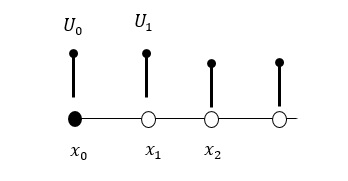
\includegraphics[scale=0.7, trim = 10mm 0mm 15mm 0mm,
clip]{./Figures/2-CauchyProblem/BC.jpg}
\caption{Boundary conditions}
\end{figure}

In a general way, any boundary condition can be written as: 
$$
F(u(x))=g;\;\; \text{if} \:\: x \in \delta\Omega \rightarrow u_0=f(u_1,u_2,
u_3,\ldots, g) $$

So, the problem has been transformed from a continuous function $u(x,t)$ to a
discrete distribution of values of this function $u_j(t)=u(x_j,t)$; which are
now the unknown quantities. Then, the problem has $m+1$ values to be
determined.\\

b) Cauchy problem \\

Once the spatial discretization is done we get a Cauchy problem: 

$$
\left(\frac{\delta u}{\delta t}\right)_j= \frac{k}{\rho \cdot c_p }\cdot {\Delta x^2} \cdot ( u_{j-1}
-2 \cdot u_{j} +u_{j+1})\\
$$

Or more generally, for any given interpolation order, $2p+1$: 

$$
\left(\frac{\delta u}{\delta t}\right)_j= f(u_{j-p},\ldots u_j, \ldots
u_{j+p})\\
$$

$$
+IC
$$

Where the unknown variables are the components of the vector $U=[U_0, U_1\ldots
, U_m]$. To continue from here, we can use the same routine as the one defined in the previous examples. \\


As we can see this process is not easy. However, using the appropriate software
tools the most part of the diffculty can be hidden. The combination of the
spatial discretization library \footnote{see High Order Finite Differences
manual (HOFD\_manual)} and the Cauchy Problem solver, complex problems can be
set to work.\\

\newpage

The process for solving a PDE problem can be summarized in the
following chart: \\

\begin{framed}
\textbf{\large PDE problem}\\
\small{

	\framebox[3.5cm]{Equations}% 
	$\rightarrow$
	\framebox[4cm]{Spatial \\ discretization}% 
	$\rightarrow$
	\framebox[1.8cm]{\textbf{System}} 
	$\iff$
	\framebox[3cm]{Cauchy problem}\\
	
	\framebox[3.5cm]{ $\begin{cases}
	\frac{d\mathbf U}{dt}={\mathscr{L}}( \mathbf U,
	t, \mathbf x)\\ 
	+IC; +BC
	\end{cases}$}% 
	$\rightarrow$
	\framebox[4cm]{ $ \begin{cases}
	 \mathbf{U}(x_j,t) \rightarrow u_j\\ 
	I_j = I_j (u_j, x) \end{cases}$}% 
	$\rightarrow$
	\framebox[1.8cm]{ $ \begin{cases}
	F(u_j,t)\\ 
	+BC
	\end{cases}$} 
	$\iff$
	\framebox[3cm]{ $\begin{cases}
	\frac{d\mathbf u_j}{dt}=F(u_j,t)\\ 
	+IC
	\end{cases}$} \\

}
\end{framed}


\hspace{5cm}

These examples show the strategy we need to follow in order to solve a
differential equation problem. The most important thing to remark is how the
described procedure can be used independently of the particular problem. This
way a whole set of subroutines and modules can be used, saving the effort of
developing special software for each application. \\

Another important characteristic of this method is that we can change the
current operation schemes without altering the whole project structure. For
example, we may want to vary the interpolating polynomials (and its order); but
it will not change the following operations, since the action is
\textit{encapsulated}. The same can be said about the temporal schemes: its
operations are held inside the Cauchy module, and this is the only thing that
our program \textit{needs} to \textit{see}.\\

\vspace{1cm}

So let's picture our program as a set of  inter-connected black boxes. Each box
is called with some input arguments, performs some operations inside and gives
some outputs. The \textit{boxes} are structured in layers as we have seen in the
chart in the third page. Each layer is independent to the others, has its own
internal procedures, inputs and outputs. The information does not travel
transverely, that is why each layer can work independently. \\

The API rules the information transference between layers, and each layer has
its own. In this manual we are focused in the Cauchy Problem API, but an API is
defined for any single layer.\\

The API is important in order to use the operators and procedures held
in the lower layers. To know the API is basic to write the application layer of
any code. 
\\

\newpage
\section{Software implementation}

In this section we are going to deal with the construction of the application
layer of the program.
Since some examples have already been presented, the objective right now is to describe the process in a generic
way.\\

Let's assume we want to solve the following PDE 2D problem: 
$$
\mathscr{L}\left(\frac{d^n \mathbf U}{dt^n}, \frac{d^{n-1} \mathbf
U}{dt^{n-1}}, \ldots, \frac{d^r \mathbf U}{dx^s dy^{r-s}}, \ldots,
\mathbf U, x, y, t\right)=0 \hspace{1cm} \forall(x,y)\in\Omega; \;\; t\geq t_0
$$

According to initial and boundary conditions, which in the most general case
can be arbitrary. \footnote{Dirichlet and Neumann conditions have already been 
implemented in the software application.

$$
Neumann: \:\: \left(\frac{\delta u}{\delta
x}\right)_{x=a} = P; \hspace{1cm} a\in \delta \Omega$$


$$
Dirichlet: \:\: u(x=a)=Q; \hspace{1cm}  a\in \delta \Omega
$$\\

Initial value problems with different boundary conditions that the ones described above 
these lines can as well be resolved using the software. However, a function should be included 
for solving the specific condition. 
We will deal with this a bit later. 
}\\

The solution of the problem is: 
$$ \mathbf U = \mathbf U(x, y, t) $$\\

However, the numerical solution is only known in some points (\textit{spatial discretization}) and in
some discrete instants (\textit{temporal discretization}).\\

Therefore, the solution will be something like this (it could vary depending on the problem's dimension):
$$ \mathbf U = \mathbf U_{ij}^n $$\\

Where $\mathbf{U}$ is a vector containing the unknown variables of the problem, which are now known
in every $(i,j)$ point, in the time step $n$. \\

This section will guide the reader throught the different actions that are
needed for the program to work propperly. Basically the information to give
the problem is: \\
\begin{itemize}
  \item The problem we want to solve. This is called {\bf{system}}.
  \item The initial conditions. 
  \item The time domain.
  \item The temporal scheme we want to use in order to solve the problem.
  \item The outputs and graphics we want the program to build. 
\end{itemize}

\newpage


\subsection{Cauchy Problem API}

The routine for the temporal integration of the problem is defined as seen in
the following box: \\

\begin{blueframed}
\begin{lstlisting}
subroutine Cauchy_Problem_Solution( Domain,  Initial_C, &
				System, Scheme, Outputs)
        
     procedure (Temporal_Domain)  :: Domain 
     procedure (Initial_Condition) :: Initial_C
     procedure (System_ODES) :: System
     procedure (Temporal_Scheme), optional :: Scheme
     procedure (ODES_Outputs), optional :: Outputs 
     
     
\end{lstlisting}
\end{blueframed}

So, these items have to be defined: \textbf{time}, \textbf{initial
condition}, \textbf{system}, \textbf{temporal scheme} (optional)
and \textbf{outputs}(optional), as we have seen in the
previous section. 
\\

\vspace{1cm}


Before continuing with the explanation of the API, a special remark should be
done in order to understand how the program works. \\

The first step in the process will be the transformation of the equation (or
equations) to a first-order temporal derivative form. We have already practised
this with the previous examples, however we are now going to apply the procedure
to an EDP problem. \\

For the program to work equally for any given problem (ODE, PDE: 1D, 2D ...),
all the unknown variables, and its temporal derivatives will be stored in a pointer on
the form:
$\mathbf{U}=\mathbf{U}(:)$ \footnote{In fact it is a vector but the definition
as a pointer will bring some advantages in terms of memory allocation and
access to the stored data}.
The advantage of proceeding this way is that there is no need to define different procedures depending on the problem's
dimension.\\

An example is proposed in order to bring some light to what we are talking
about: for the sake of simplicity, let us consider 1D wave
equation:

$$
\frac{d^2 \mathbf{X}}{dt^2}-c^2\cdot\frac{d^2 \mathbf{X}}{dy^2}=0
$$\\

Where $\mathbf{X}$ is a vector containing the function value in the points of
the discretization. Therefore: $$\mathbf{X}=\mathbf{X}(0:N_y)$$ \\

The transformation to a first order derivative form will give: 
$$
\frac{d}{dt}
\begin{bmatrix}
X\\
\dot X
\end{bmatrix}= \begin{bmatrix}
\dot X\\
c^2 \cdot X_{yy}
\end{bmatrix}
$$\\

The left hand of the equation is to be defined as a vector to fit with the usual
Cauchy problem definition: 
$$
\mathbf{U}=[\mathbf{X}(0:N_y) \:\: \mathbf{\dot X}(0:N_y)]; 
$$\\

So the vector $\mathbf{U}$ has dimension: $2\cdot(N_y+1)$.\\

\begin{framed}
$$
\mathbf U = [X \dot X]
$$
$$
\frac{d \mathbf U}{dt}= \mathbf F(\mathbf U) \longrightarrow 
\begin{cases}
F_1=\mathbf{U}(m+1:2\cdot m); \hspace{1cm} m=N_y+1\\
F_2=c^2\cdot X_{yy}
\end{cases}
$$
\end{framed}


This procedure can be generalized to n-th derivatives: 
$$
U(1:m)=\mathbf X 
$$
$$
U(m+1:2\cdot m) =\mathbf{\dot X}
$$
$$\ldots$$
$$
U \left(n\cdot m+1: (n+1)\cdot m \right)= \frac{d^n \mathbf X}{dt^n}
$$\\

The dimension of the vector $\mathbf{U}$ will be $(n+1)\cdot m$ where $n$ is the
order of the temporal derivative and $m$ depends on the problem dimension. For
an ODE, $m=1$, (go back to the mass-spring-damper example to clarify ideas);
while for a PDE we have:
$$ 1D: \:\: m=N_x+1 $$
$$ 2D: \:\: m=(N_x+1)\cdot (N_y+1)$$
$$ 3D: \:\: m=(N_x+1)\cdot (N_y+1) \cdot (N_z+1)$$\\

Generally speaking, $m$ is the total amount of unknown variables we have in our
problem. Then, the vector $\mathbf{U}=\mathbf{U}(:)$ is completed with its
temporal derivatives depending on the temporal order of the problem. \\

These operations must be done, usually by hand, before starting working with the
software.
It is important to keep this structure in mind in order to write the fortran file
properly, as it will be the key to the system definition and also the initial
condition statement should be written according to this syntax.\\

\newpage





\section{Application layer}

This section is the most important part of the manual. Here, the essential
information is presented for the program to use the procedures of the library.
The syntax and structure of the routines must be respected carefully. \\

The software we need to build in order to solve our problem is very simple in
terms of programming. We just need to define the system (described by an
equation or a set of equations), the time and space domain and the initial and
boundary conditions. The output information we want the software to build
can be also specified (otherwise the program will use the default settings). \\

The key of our software is the multi-layered structure. Therefore, specific
syntax and procedures must be used in order to use the program's modules
(contained in the lower layers).
\\

\vspace{1cm}

The software {\bf must} have the following structure according to the API of
the library:\\

\begin{blueframed}

\begin{lstlisting}
module [generic problem]

	!Declaration of needed modules
	use Cauchy_Problem
	use [...]  !spatial discretization, if needed
	
	!Declaration of variables
	implicit none
	private
		real:: ...
	
	public :: test_problem
	
	contains
	
		subroutine Time_Domain(Time)
			[...]
		end subroutine
		
		subroutine problem_IC (t0,U)
			[...]
		end subroutine
		
		subroutine System(t,U,F)
			[...]
		end subroutine
		
		subroutine outputs(t,U,S)
			[...]
		end subroutine
		
		subroutine Test
			[...]
		end subroutine

end module
\end{lstlisting}
\end{blueframed}

The system definition is compulsory (otherwise we do not have a problem). In a
Cauchy problem, time and initial condition must be declared. \\

The output subroutine is optional. If there is not a specific assignment the
program will use the default settings.
\\

Finally, the test subroutine must be included. This subroutine allows us to
launch the problem resolution and to get the results. Also, we can check the
results in order to validate the program.\\

\subsection{Variable declaration}

First of all we are going to declare all the variables that will be used
\textit{inside} the module. These variables will be declared after the
\textbf{private} statement. \\

As an example, the variables for a 2D generic problem might be: 

\begin{blueframed}
\begin{lstlisting}
 implicit none 
 private 

 	real, save :: t0 = 0., tf = 7.5 
 	integer, save :: Nx = 20, Ny = 20, Order = 8; 
 	real, save, allocatable :: x(:), y(:) 
 	integer, save :: N   !time steps
 	
 	!any other variables needed for the problem definition 
 	!or plotting the results
 
  public :: Test_2D
\end{lstlisting}
\end{blueframed}

Here we can see how the time limits are specified, also the number of spatial
divisions we want ($N_x$, $N_y$) and the interpolation order (set to $8$ in
this example, as we want to test high order schemes).\\

The $test$ subroutine is declared public. This way it can be called from
\textit{outside} the module. \\

The reason for remarking the difference between public and private arguments is
for the program not to become a mess if some variables interact between modules.
This way the information is classified and the access to the operators is
limited. \\

The save statement is used to keep the value of the variables after a function
call. Then the variable is initialized with its initial (saved) value. \\

\newpage



\subsection{Time domain}

The time must be specified as a pointer according to the following structure: \\

\begin{blueframed}
\begin{lstlisting}
subroutine Time_Domain( Time ) 
 real, pointer :: Time(:) 
 
    integer :: i 
    
     N = 6000      !Time steps 
     allocate ( Time(0:N) ) 

     !example
     Time = [ (t0 + (tf-t0)*i/(1d0*N), i=0, N ) ]  
 
end subroutine 

\end{lstlisting}

\end{blueframed}

An example has been included just to help the comprehension of this routine.
Please note that any other time partition can be made.\\

The $t_0$ and $t_f$ values have been specified  before in the variable
declaration.\\

\subsection{Initial condition}

This subroutine will assign the initial value of the components of the vector
$\mathbf{U}$.\\

\begin{blueframed}
\begin{lstlisting}
subroutine  problem_IC( t0, U)
   real, intent(in) :: t0 
   real, pointer :: U(:)

	 allocate( U((n+1)*m) )
	!initial value of the vector U 
	
end subroutine 
\end{lstlisting}

\end{blueframed}

Note that the vector should be allocated first. Its dimension will be
$(n+1)\cdot m$. When dealing with PDE problems ($m > 1$), the grid should be
initialized before giving values to $\mathbf{U}$.\\

\newpage 

A 2D example can be written this way: \\

\begin{blueframed}
\begin{lstlisting}
     integer :: M 
     
      M = (Nx+1)*(Ny+1); 

    allocate( x(0:Nx),  y(0:Ny), U(2*M) ) 

	call Grid_Initialization( "uniform", "x", Order, x )
	call Grid_Initialization( "nonuniform", "y", Order, y )
        
    call IC(Nx, Ny, U(1:M), U(M+1:2*M) ) 
\end{lstlisting}
\end{blueframed}

The routine {\textit{Grid\_Initialization}} has already been
described in the HOFD manual. Please remember that $x$ and $y$ are assumed in
the interval $[0,1]$. Any other space domain (square) can be defined multiplying
by the corresponding coefficients.\\

In the example a second subroutine ($\textit{IC}$) is used to assign the values
to the $\mathbf{U}$ vector components, but it is not compulsory to do it like
this (it can be assigned directly, but be careful with the assignment because
$\mathbf{U}$ contains the values $U(x,y,t)$ and sometimes also its derivatives, all sorted in a single row).
\\

\subsection{System definition}


\begin{blueframed}
\begin{lstlisting}
subroutine System(t,U,F)

	real, intent(in)  :: t
	real, intent(inout)  ::  U(:)
	real, intent(out) :: F(:)
	
	![the function assignment comes here]
	!F=f(U,t)
	
end subroutine
\end{lstlisting}
\end{blueframed}

Sometimes the system definition involves only ODEs (as examples, we have
already seen a mass-spring-damper system and the Lorenz attractor). These
problems do not involve the spatial discretization and the program can go
straight to the temporal discretization.\\

More generally speaking, we might need spatial discretization to solve our
problem. Go back to HOFD manual to check the tools and its syntax, if needed. \\

Please remark that $\mathbf{F}$ comes from: 
$$
\frac{d \mathbf{U}}{dt}= \mathbf{F}
$$

So it has the same structure and dimension as $\mathbf{U}$.\\

\subsection*{Examples}

Somes examples are going to be presented in order to clarify the ideas and show
how the system is to be defined.

\subsubsection*{ODE: mass-spring-damper}

\begin{blueframed}
\begin{lstlisting}
subroutine mass-spring-damper(t,U,F)

	real, intent(in)  :: t
	real, intent(inout)  ::  U(:)
	real, intent(out) :: F(:)
	
	real, parameter :: M=1.0, D=1.0, K=1.0
	real :: P
	
	P= 1.*sin(pi*t)  !example
	
	F(1)=U(2)
	F(2)=(P-D*U(2)-K*U(1))/M	
	
end subroutine
\end{lstlisting}
\end{blueframed}

A detailed example of this system is explained afterwards.\\

\subsubsection*{ODE: Lorenz attractor}

The following proposed example is the Lorenz attractor. The complexity is a
bit higher, as it is a non linear system, sometimes chaotic depending on the
model parameters.

\begin{figure}[H]
\centering
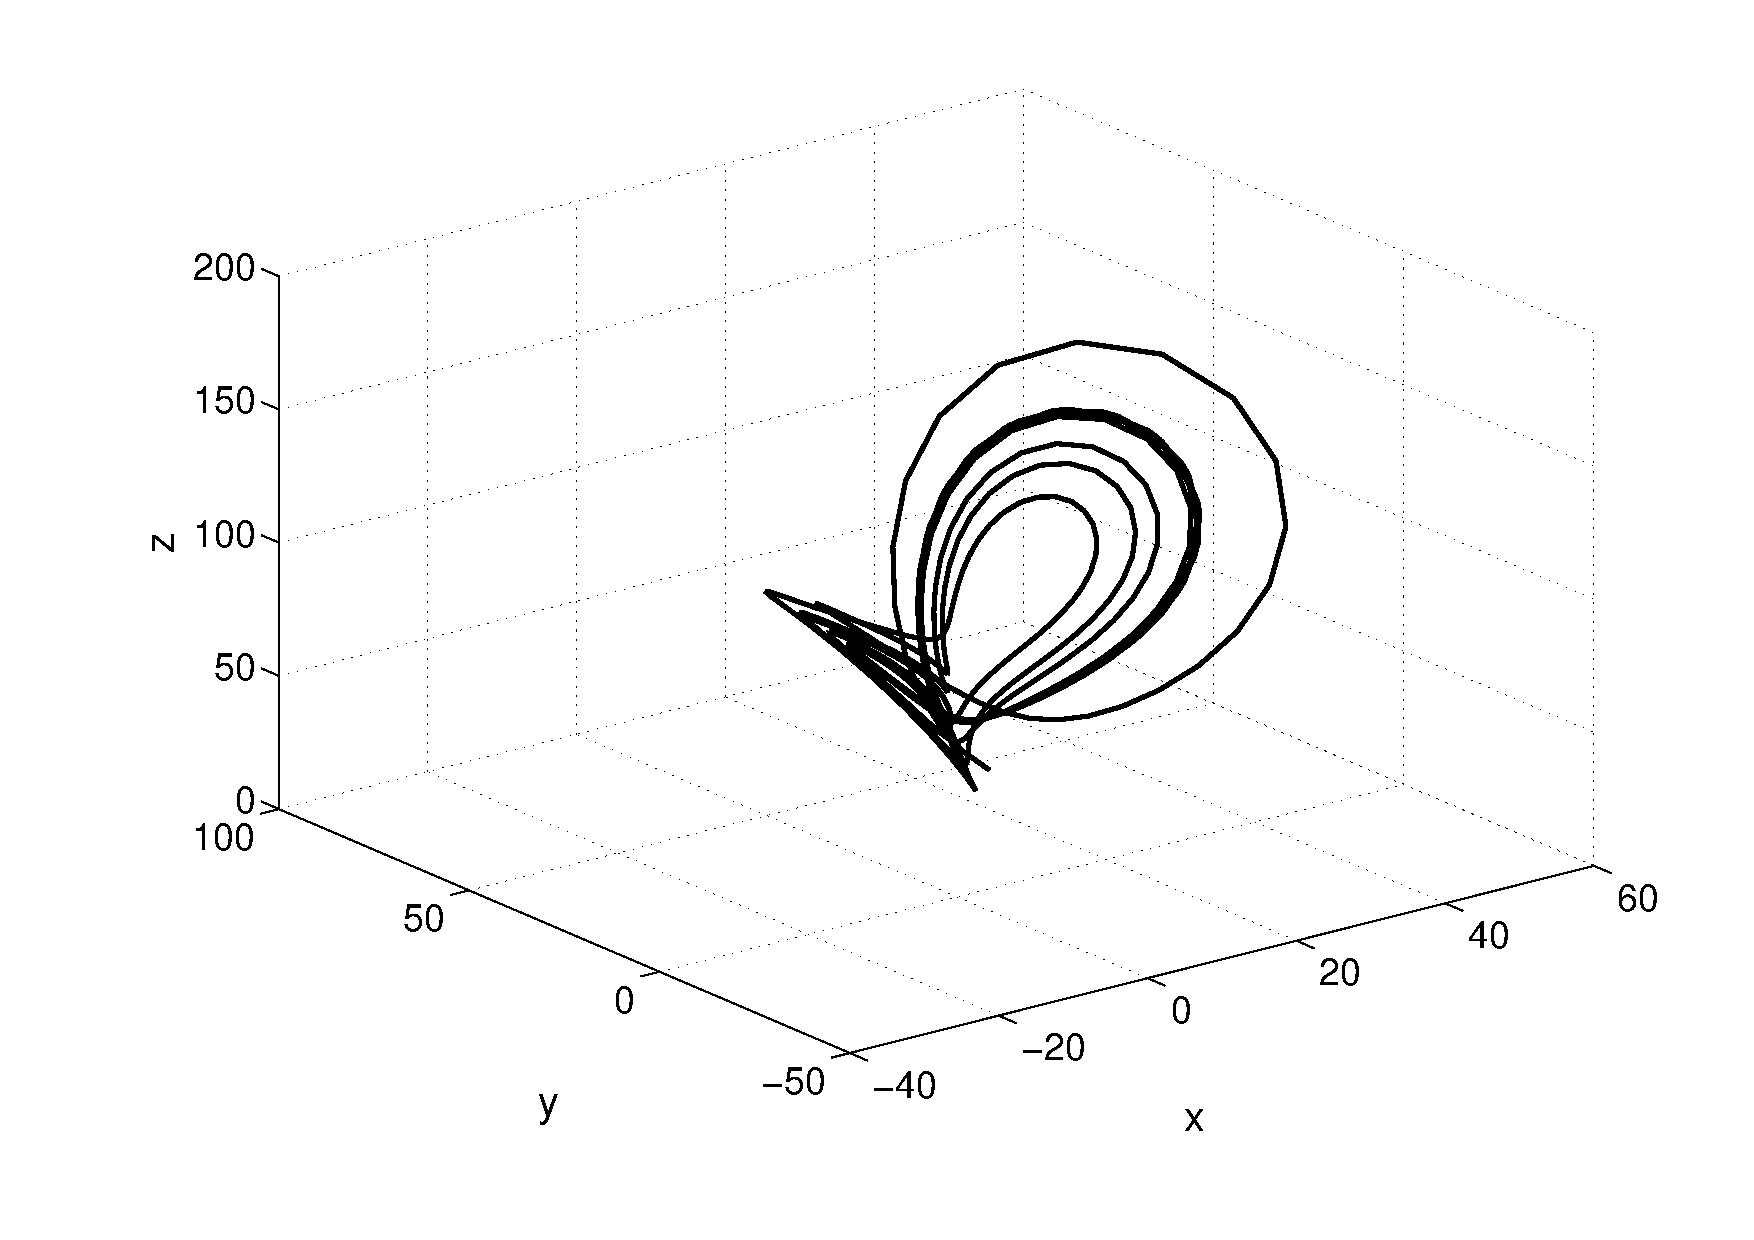
\includegraphics[scale=0.4, trim = 20mm 0mm 0mm 0mm, clip]
{./Figures/2-CauchyProblem/lorentz_3.pdf}
\caption{The Lorenz attractor.}
\end{figure}

The system routine for this problem should be written as follows: 

\begin{blueframed}
\begin{lstlisting}
subroutine  Lorenz_attractor(t, U,  F)        
    
     real, intent(in)  :: t
     real, intent(inout)  ::  U(:)
     real, intent(out) :: F(:)
      
     real :: x, y , z
	  
	 x = U(1); y = U(2); z = U(3)   

    	 F(1) =   a * ( y - x ) 
	 F(2) =   x * ( b - z ) - y 
	 F(3) =   x * y - c * z   

end subroutine 
\end{lstlisting}
\end{blueframed} 


As cuorisity, the following figures present the results of the system described
above. The results can be very different depending on the parameters ($a$, $b$,
$c$) of the system. 

\begin{multicols}{2}

\begin{figure}[H]
\centering
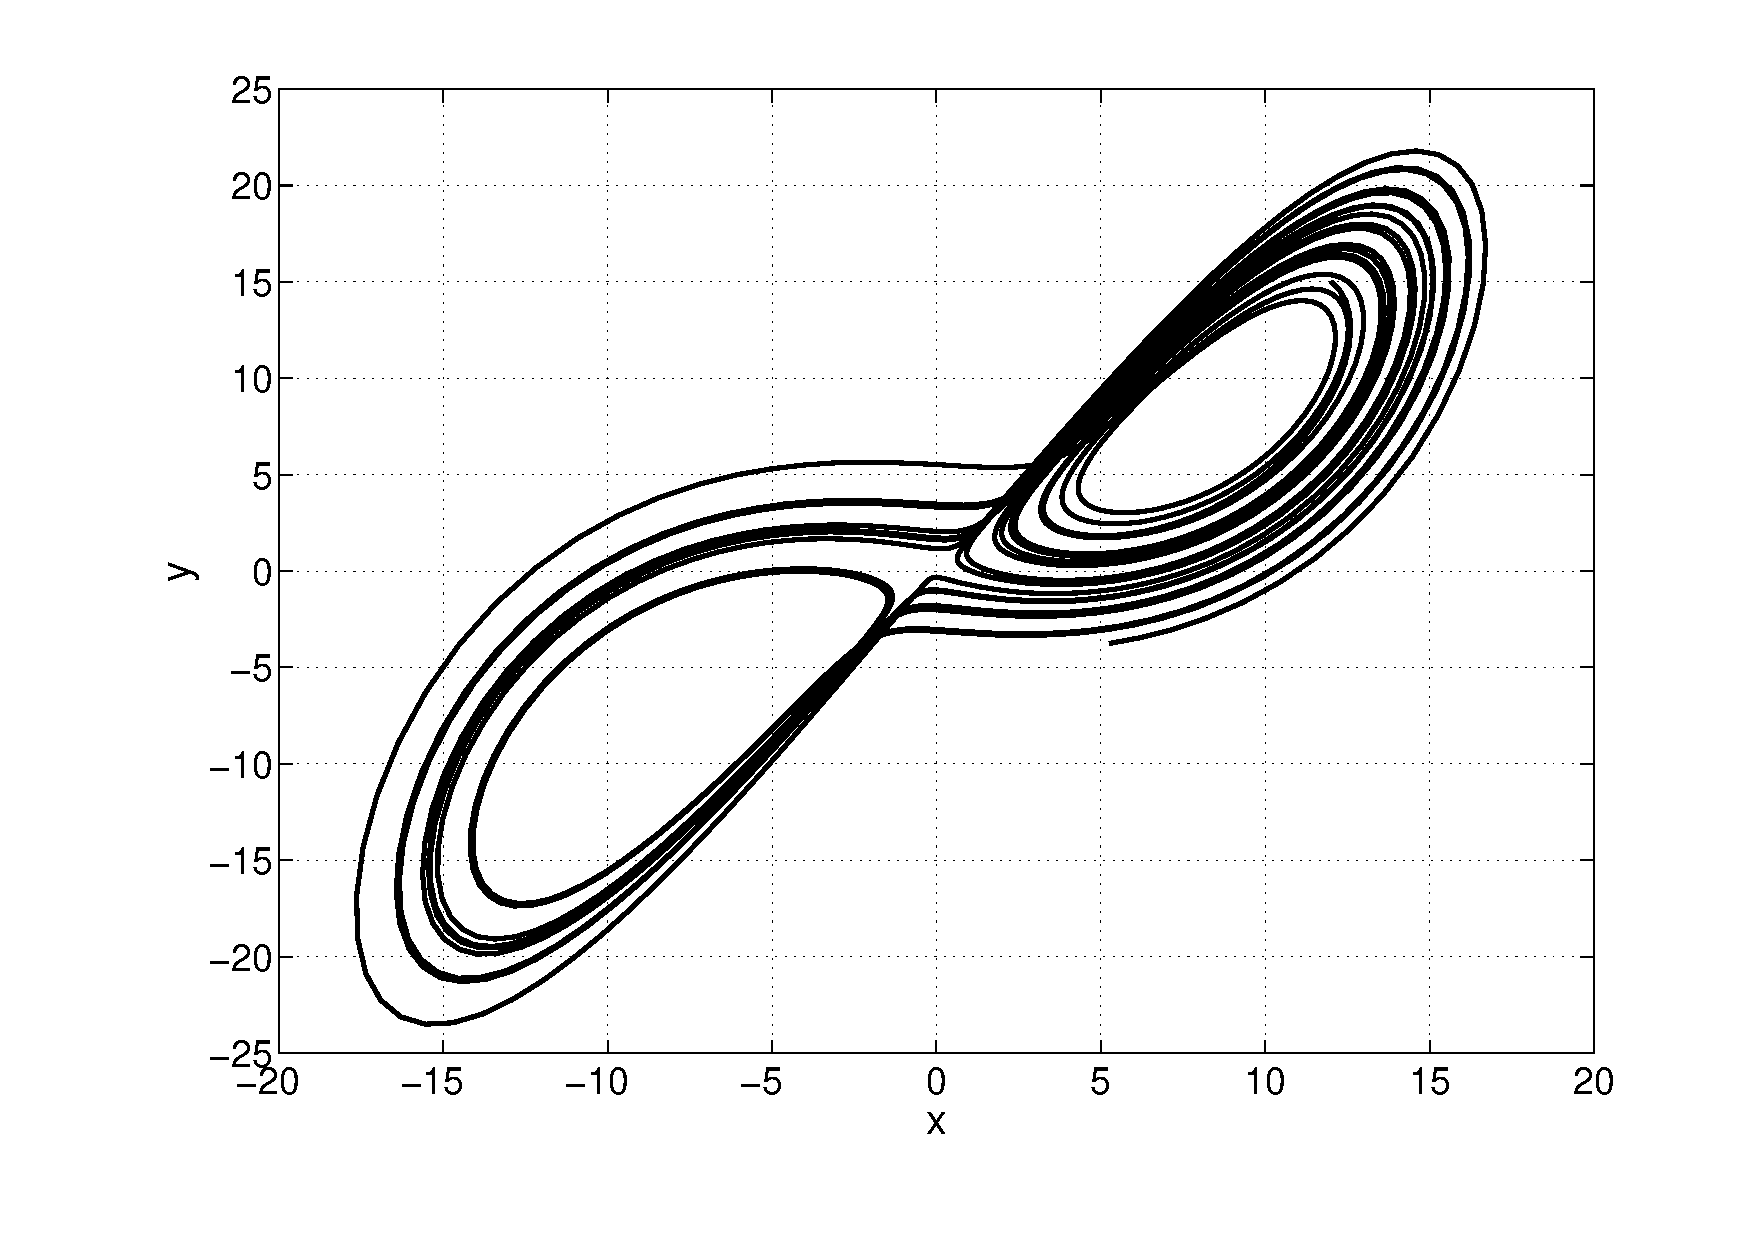
\includegraphics[scale=0.3, trim = 20mm 0mm 0mm 0mm, clip]
{./Figures/2-CauchyProblem/lorentz_xy.pdf}  \caption{2D plot ($x \:\: vs. \:
y$) of the Lorenz attractor with $a=10$, $b=28$ and $c=2.67$.} 
\end{figure}

\columnbreak

\begin{figure}[H]
\centering
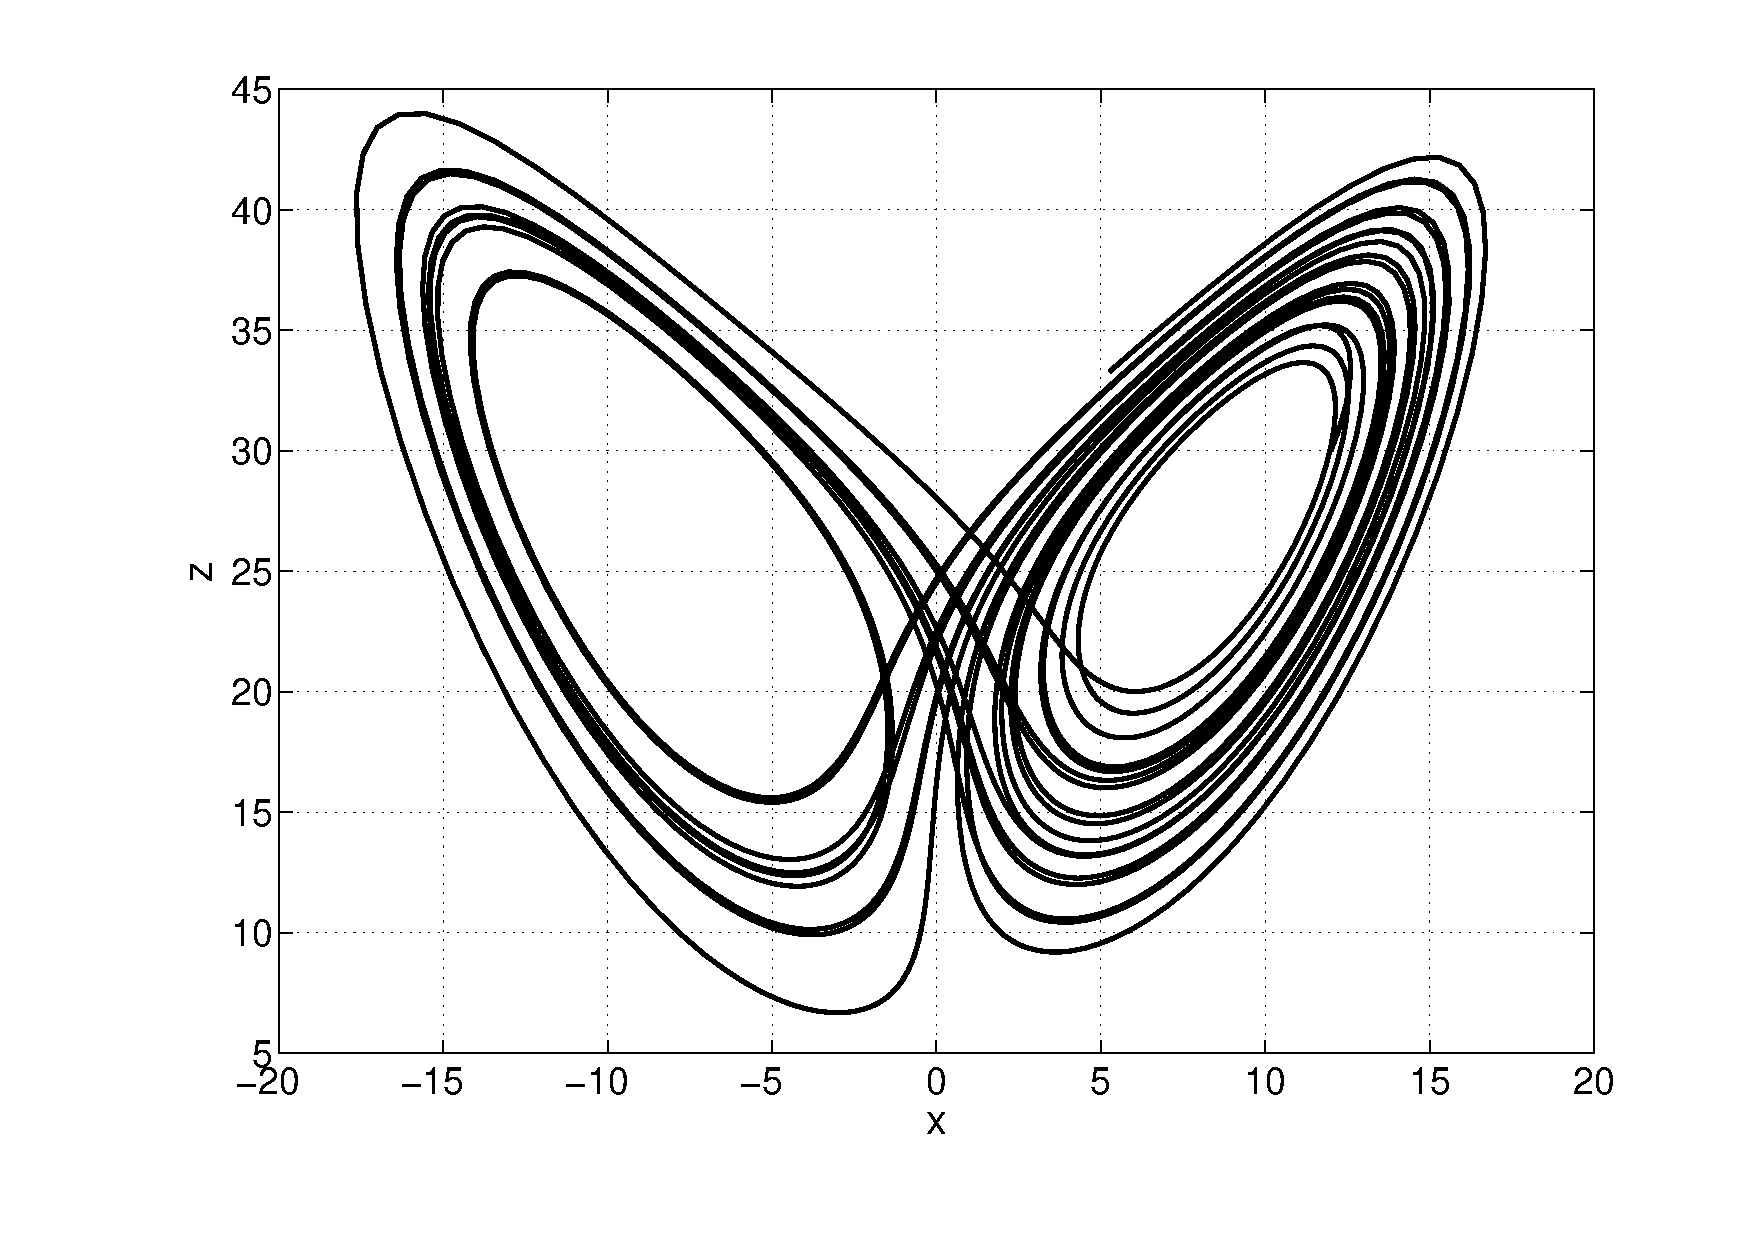
\includegraphics[scale=0.3, trim = 20mm 0mm 0mm 0mm, clip]
{./Figures/2-CauchyProblem/lorentz_xz.pdf}
\caption{2D plot ($x \:\: vs. \: z$) of the Lorenz attractor $a=10$,
$b=28$ and $c=2.67$.}
\end{figure}

\end{multicols}

\begin{multicols}{2}

\begin{figure}[H]
\centering
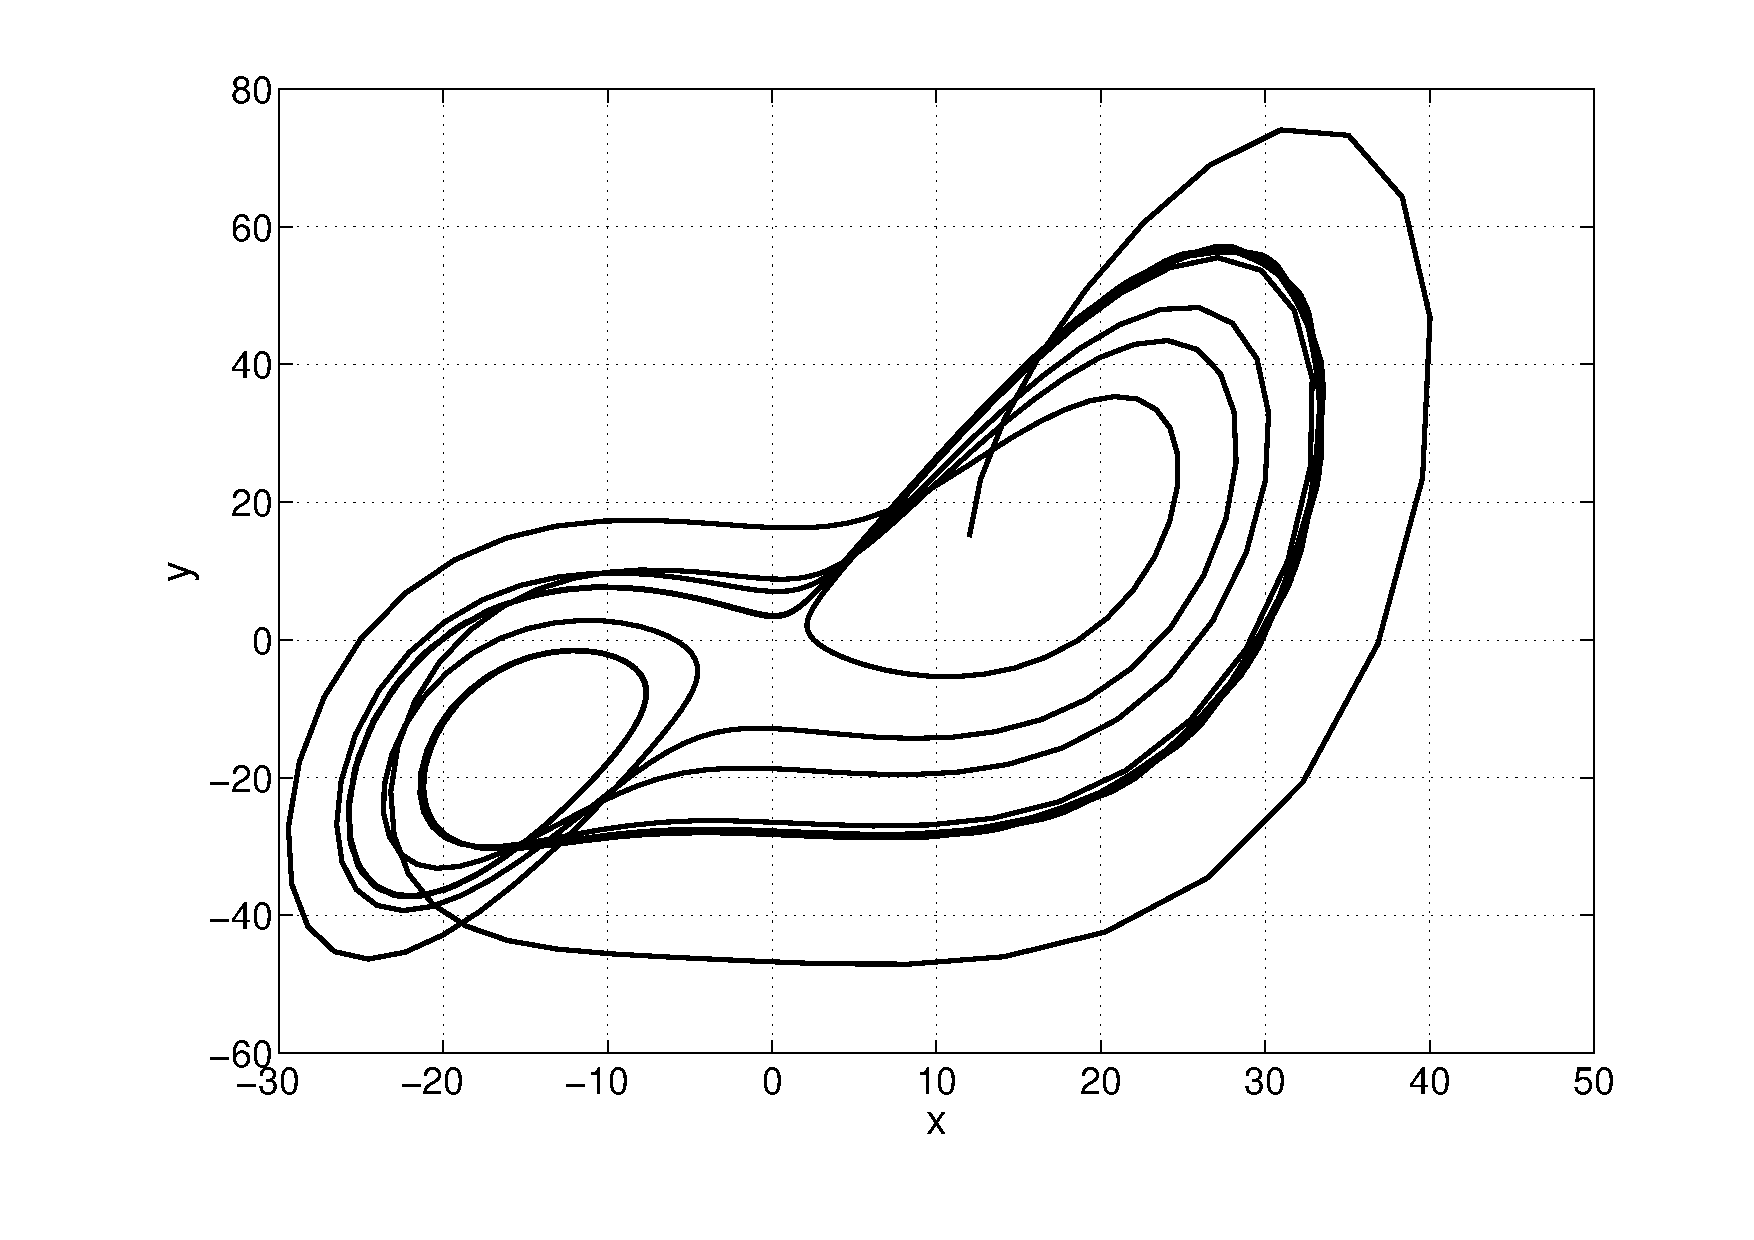
\includegraphics[scale=0.3, trim = 20mm 0mm 0mm 0mm, clip]
{./Figures/2-CauchyProblem/lorentz_xy2.pdf}
\caption{2D plot ($x \:\: vs. \: y$) of the Lorenz attractor with $a=10$,
$b=99.96$ and $c=2.67$.}
\end{figure}

\columnbreak

\begin{figure}[H]
\centering
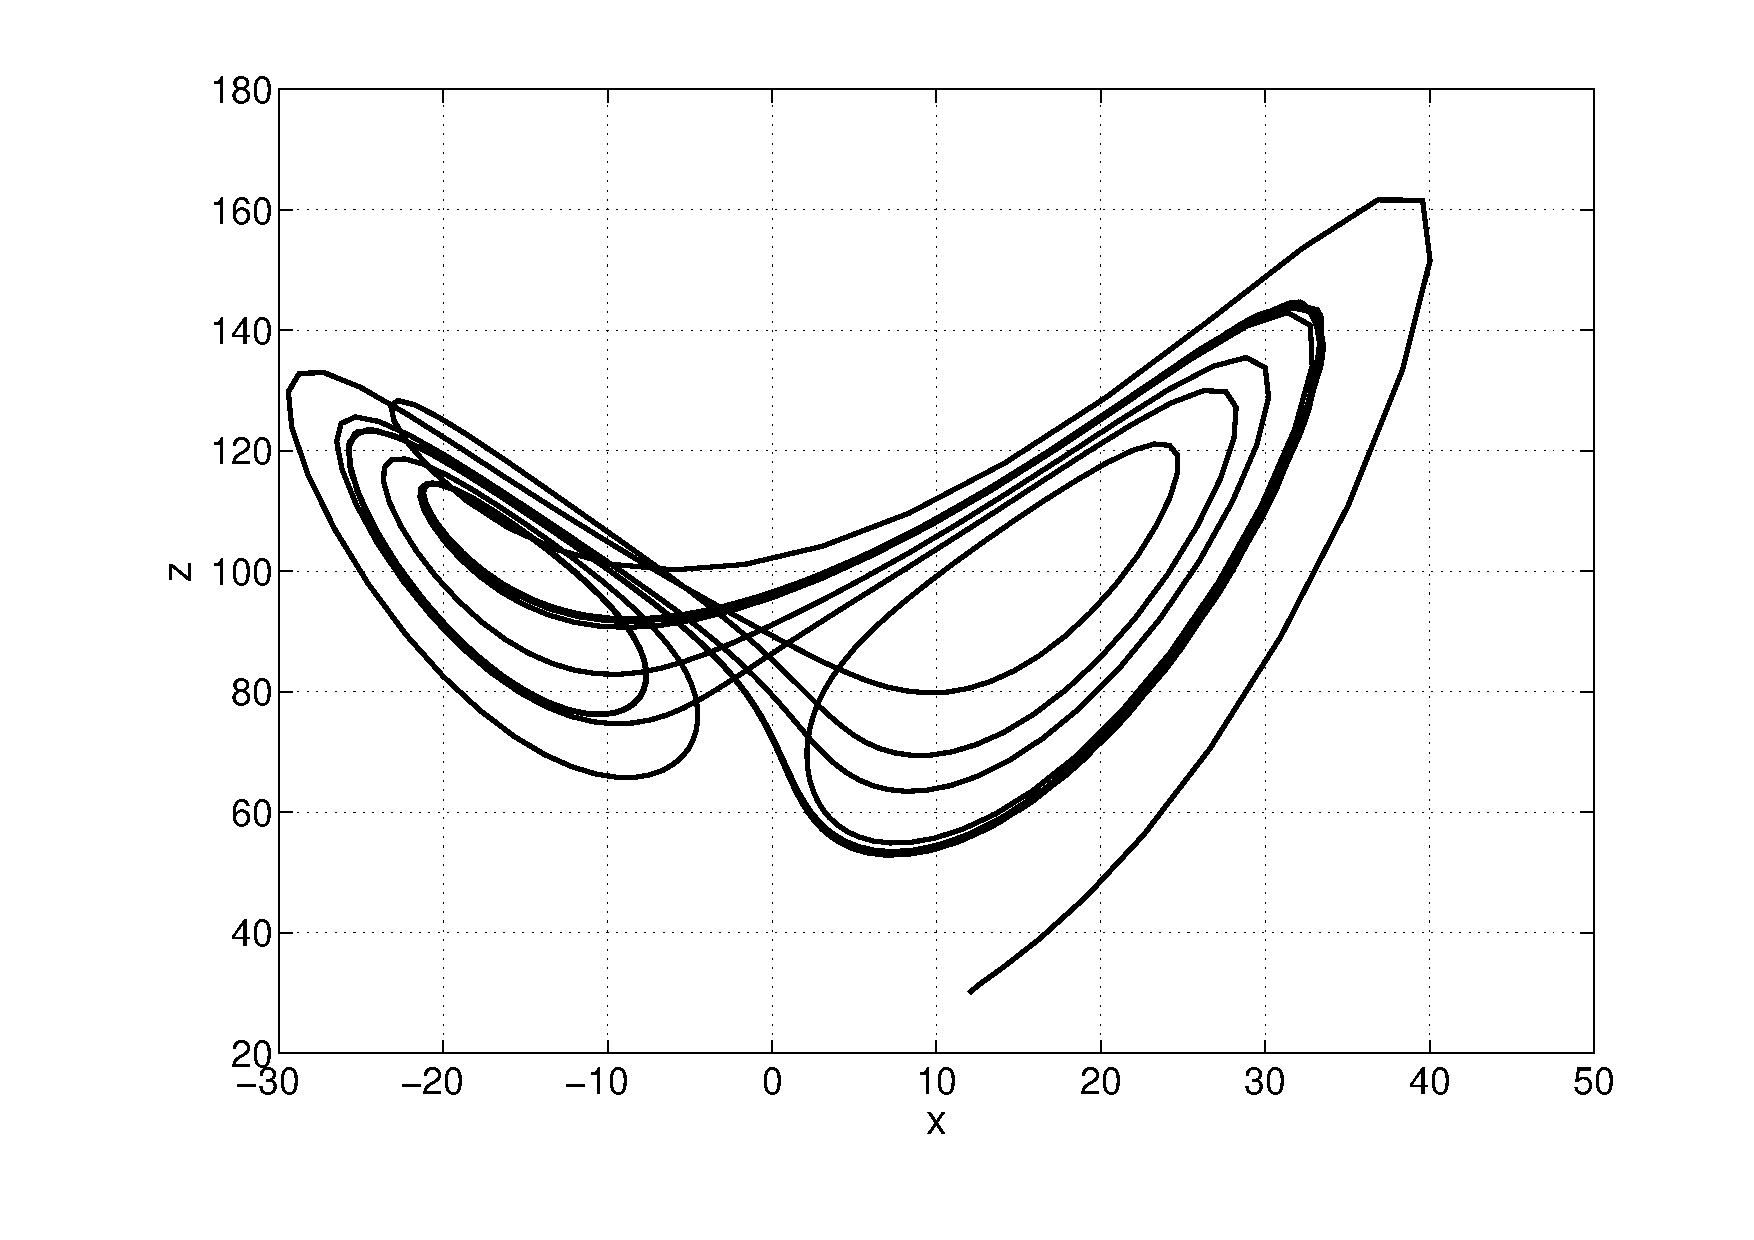
\includegraphics[scale=0.3, trim = 20mm 0mm 0mm 0mm, clip]
{./Figures/2-CauchyProblem/lorentz_xz2.pdf}
\caption{2D plot ($x \:\: vs. \: z$) of the Lorenz attractor $a=10$,
$b=99.96$ and $c=2.67$.}
\end{figure}

\end{multicols}

\newpage


\subsubsection*{EDP: Wave equation 2D}

\begin{blueframed}
{\begin{small}
\begin{lstlisting}
subroutine  Wave2D_equation(t, U,  F)            
              real, intent(in)  :: t
              real, intent(inout)  ::  U(:)
              real, intent(out) :: F(:)

  integer :: M 

  M = (Nx+1)*(Ny+1) 
 
  call Wave2D_equations(Nx, Ny, U(1:M), U(1+M:2*M), F(1:M), F(1+M:2*M)) 

contains 

	subroutine Wave2D_equations( Nx, Ny, P, W, Fp, Fw  ) 
	      integer, intent(in) :: Nx, Ny 
	      real, intent(inout) ::   P(0:Nx, 0:Ny),  W(0:Nx, 0:Ny) 
	      real, intent(out) :: Fp(0:Nx, 0:Ny), Fw(0:Nx, 0:Ny) 
	
	      real :: Pxx(0:Nx, 0:Ny), Pyy(0:Nx, 0:Ny) 
	
	 !** Boundary conditions 
	      call Newmann("x",0, P, 0.); call Newmann("x",Nx, P, 0.);
	      call Newmann("y",0, P, 0.); call Newmann("y",Ny, P, 0.); 
	
	  !** Wave equation
	      call Derivative( "x", 2, P, Pxx ) 
	      call Derivative( "y", 2, P, Pyy ) 
	
	      Fp =  W 
	      Fw =  4 * (Pxx + Pyy) 
	
	end subroutine 

end subroutine 

\end{lstlisting}
\end{small}}
\end{blueframed} 

\subsection{Temporal schemes}

The available temporal schemes are: 

\begin{itemize}
  \item Euler (\texttt{Euler})
  \item Leap frog (\texttt{Leap\_frog})
  \item Predictor-Corrector (\texttt{Predictor\_Corrector1})
  \item Adams-Bashforth (\texttt{Adams\_Bashforth} and
  \texttt{Adams\_Bashforth3})
  \item Crank-Nicolson (\texttt{Crank\_Nicolson})
  \item Runge-Kutta (\texttt{Runge\_Kutta4} and \texttt{Runge\_Kutta2})
  \item Inverse Euler (\texttt{Euler\_inverso})
\end{itemize}

The name between parenthesis is the name as it should be written in the
program in order to perform the procedure. If no procedure is specified, the
library will continue with \texttt{Runge\_Kutta4} by default. \\

For additional information about the different schemes, look into

 \textsc{\textbf{Juan A. Hern\'andez}, C\'alculo num\'erico en ecuaciones
 diferenciales ordinarias.}

\subsection{Outputs}

It is allowed to collect information from the resolution process using the
\texttt{Outputs} subroutine. \\

This procedure is called after every time step of the evolution problem, so a
great deal of data (both about the solution or the process) can be stored.\\

\begin {blueframed}
\begin{lstlisting}
subroutine Outputs(t,U,S)

             real, intent(in) :: t
             real, intent(inout) :: U(:)
             procedure (ODES_Outputs), optional :: S
             
             !...
             
end subroutine
\end{lstlisting}
\end{blueframed}

As we can see, the arguments to this routine are the time $t$ and the dependent
variable $U$. There is also an option to add a procedure, defined by the user,
to process the data. \\

As it has already been said, this routine is called after every time step of the
solving procedure, so the information can be taken (and plotted, if needed)
during the process or after the end of it. \\

Some useful commands for this routine are: 

\begin{itemize}
  \item \texttt{print*,} - It is useful in order to check the functionality of
  the process (sometimes the calculation is very long and, especially in the
  first stages of software development, we want to make sure that the program is
  working as expected, and waiting until the end of the process to check that
  something is not working might be a severe waste of time). \\
  \item DISLIN - this is a library which allows us to plot figures (quite
  rudimentary) directly from the code execution. It is useful in the same way as
  the \texttt{print} statement, but we are not going to use it for publishing
  results.

Some useful tools are \texttt{qplot( x, F, N )}, which represents N points of
the function $F=F(x)$ and \texttt{qplcon( F, Nx, Ny, NN);}, for plotting $NN$
isolines of a 2D function $F=F(x,y)$.\\

  \item \texttt{write(txt,fmt)} - this command allows the user to write the data
  in a \texttt{.txt} file that has to be defined. Also, one can choose
  the format (\texttt{fmt}) of the stored data. It is compulsory to open the
  file at the beginning:  \texttt{OPEN(UNIT=txt, FILE= 'results.txt',
  ACTION='write')} and close it (\texttt{close(txt)}), at the end. \\
  
\end{itemize}







\newpage

\subsection{Test}

The test routine is very simple: 

\begin {blueframed}
\begin{lstlisting}
subroutine test_mass_spring_damper

   call Cauchy_Problem_Solution( Domain = Time_Domain, & 
   				Initial_C =problem_IC,& 
   				System = mass_spring_damper, &
   				Scheme=Runge_Kutta4, &
    				Outputs=results)
end subroutine
\end{lstlisting}
\end{blueframed}

The \texttt{Cauchy\_Problem\_Solution} statement can be called as
well from the main program. However it is better to do it this way so the
program has its own checking tool and becomes independent from the main file. \\

If the purpose of the program is just to solve a given problem, the main file is
simple: 

\begin {blueframed}
\begin{lstlisting}
program main

    use example_mass_spring_damper

    implicit none


    call test_mass_spring_damper


end program
\end{lstlisting}
\end{blueframed}

However, for bigger structures where the resolution of the initial condition
problem is just a single step of the process, the main file might be a bit more
complicated. Anyway, the multilayered structure allows us to separate and to
work with this layer independently to the rest of the program construction.\\

\newpage

\subsection*{Results of the mass-spring-damper system}

The test case allows the validation of the routines.  The following figures
present the results obtained from two different simulations:  the conservative
system ($D=0$) and a damped system ($D=1$):

\begin{multicols}{2}

\begin{figure}[H]
\centering
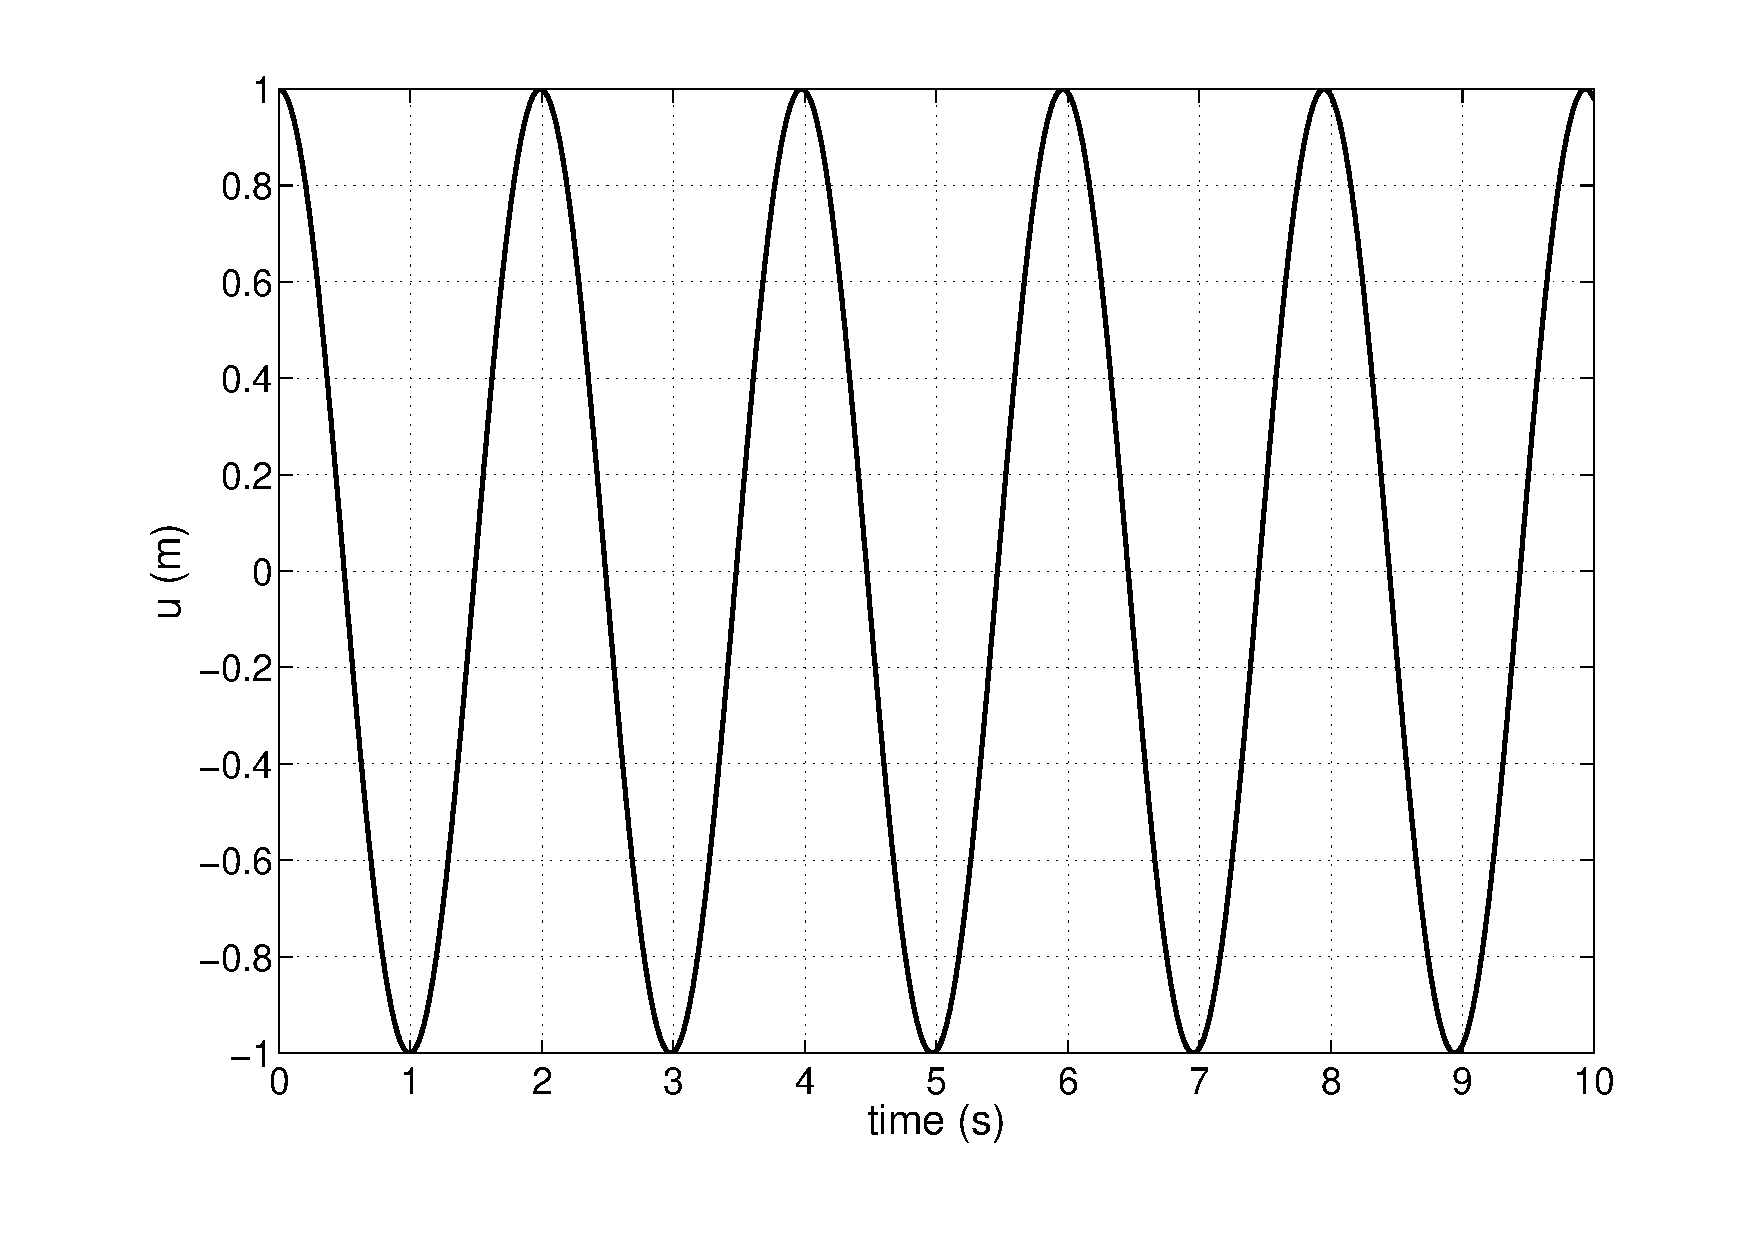
\includegraphics[scale=0.3, trim = 20mm 0mm 0mm 0mm, clip]
{./Figures/2-CauchyProblem/D=0.pdf}
\caption{Conservative system.}
\end{figure}

\columnbreak

\begin{figure}[H]
\centering
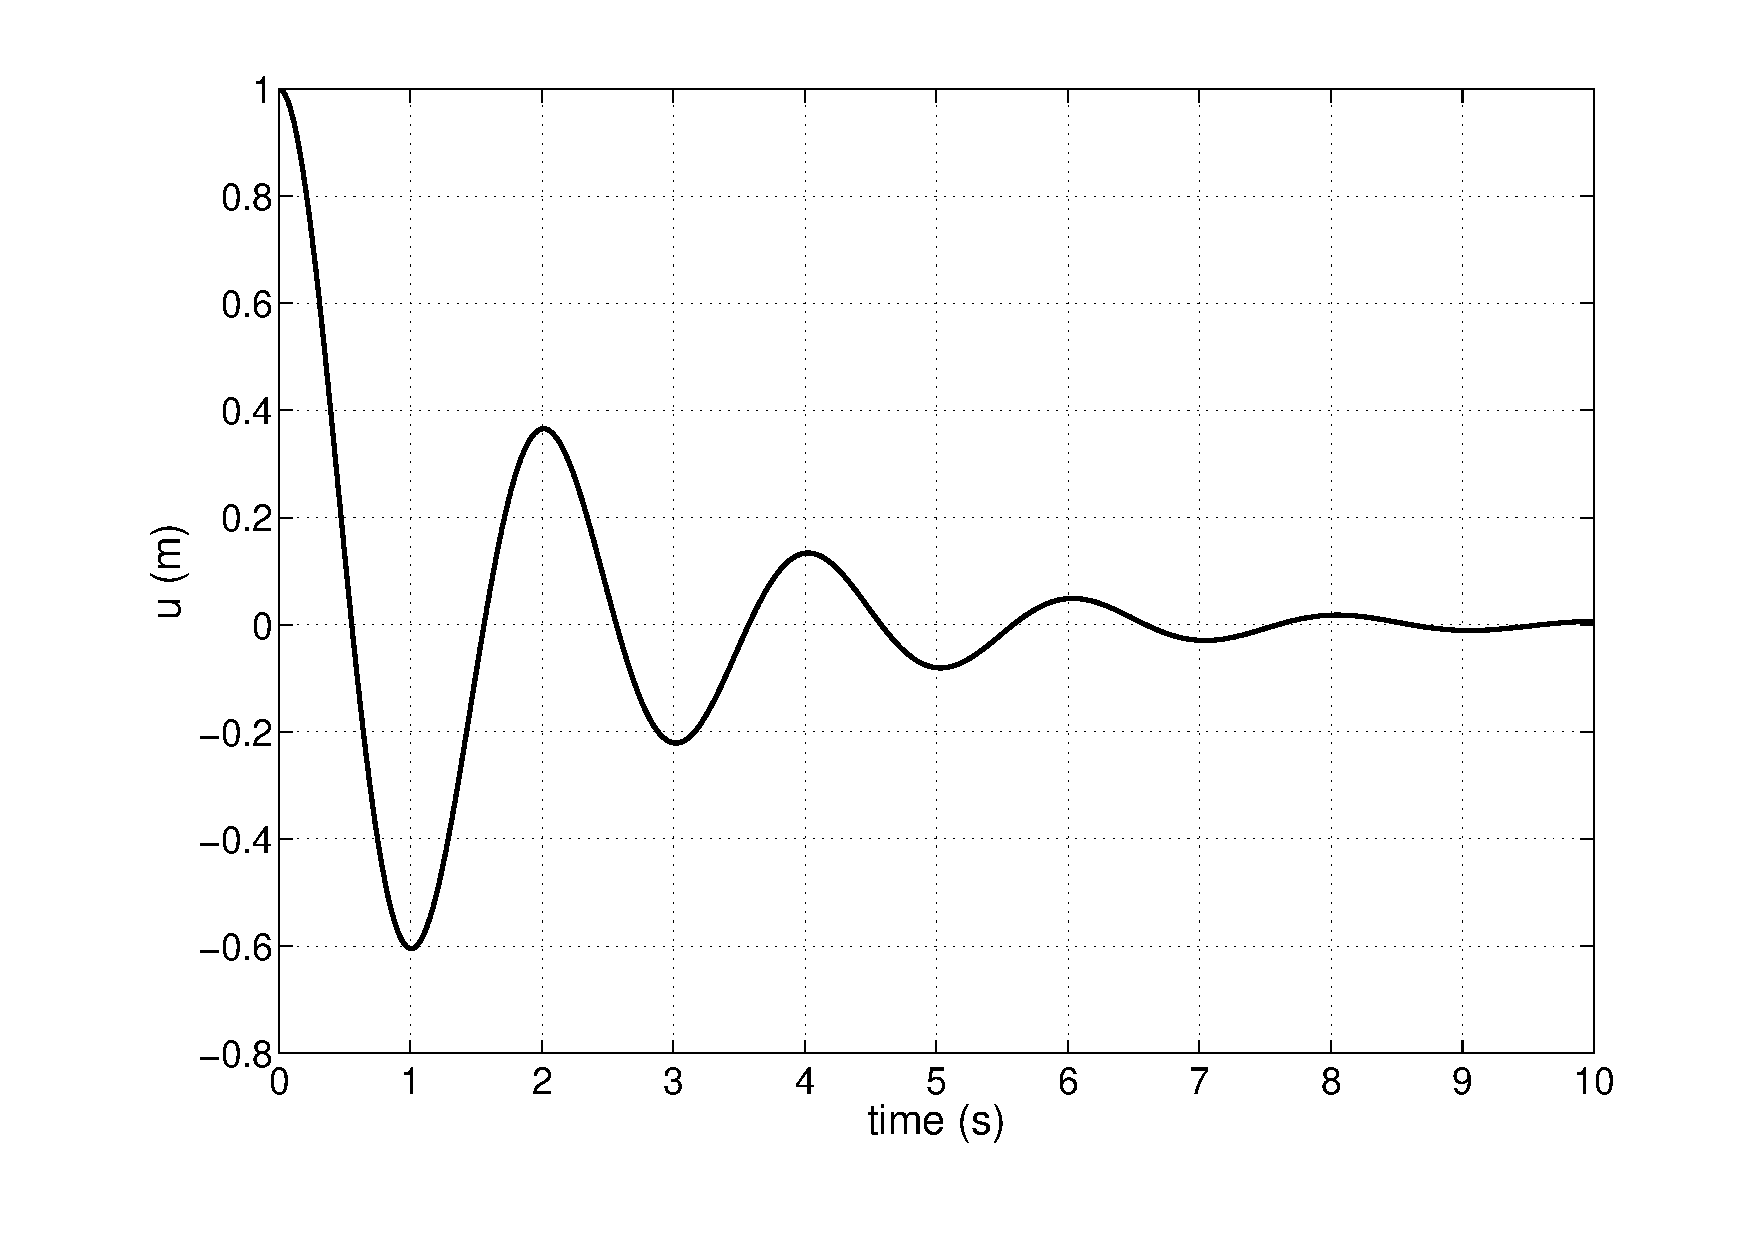
\includegraphics[scale=0.3, trim = 20mm 0mm 0mm 0mm, clip]
{./Figures/2-CauchyProblem/D=1.pdf}
\caption{Damped system.}
\end{figure}

\end{multicols}

\begin{multicols}{2}

\begin{figure}[H]
\centering
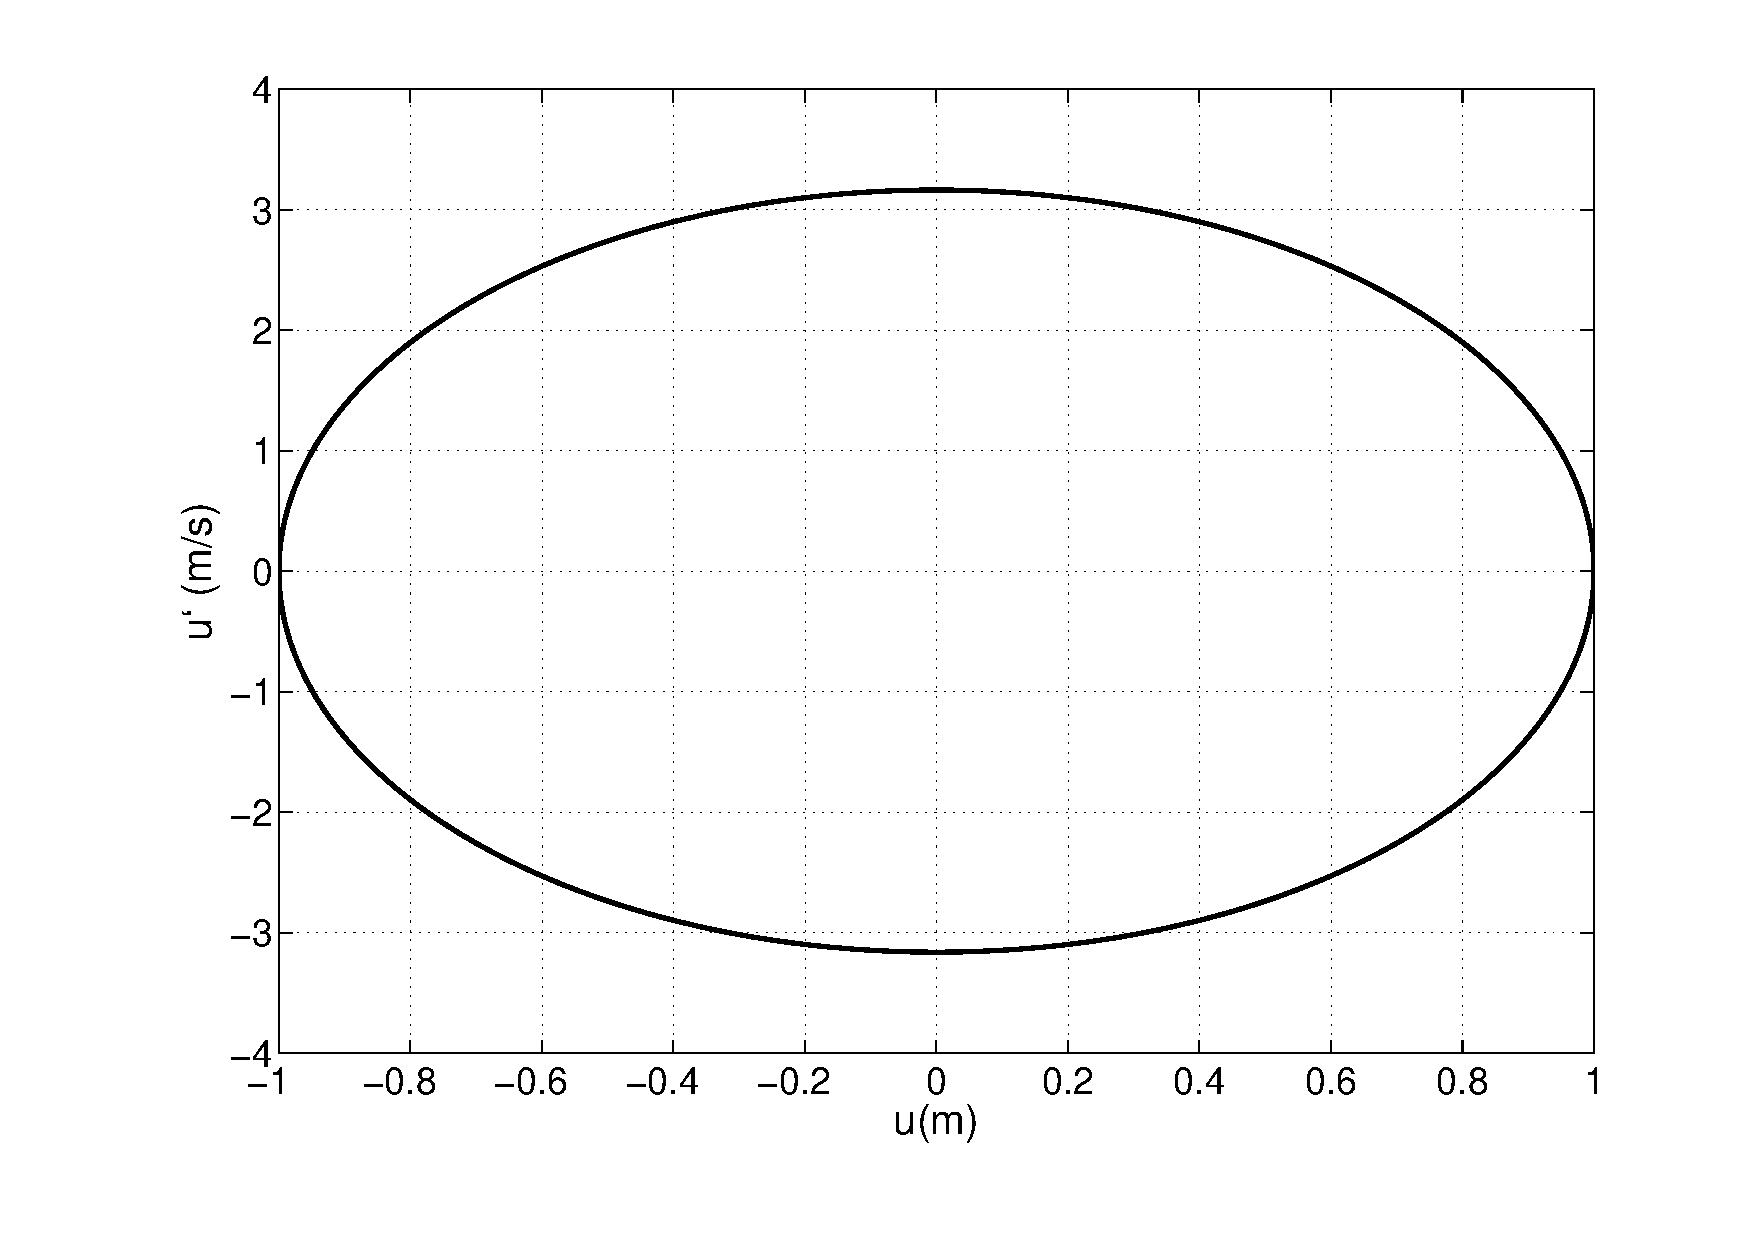
\includegraphics[scale=0.3, trim = 20mm 0mm 0mm 0mm, clip]{./Figures/2-CauchyProblem/D=0_uu.pdf}
\caption{Position ($u$) vs. velocity ($\dot{u}$) for the conservative system.}
\end{figure}

\columnbreak

\begin{figure}[H]
\centering
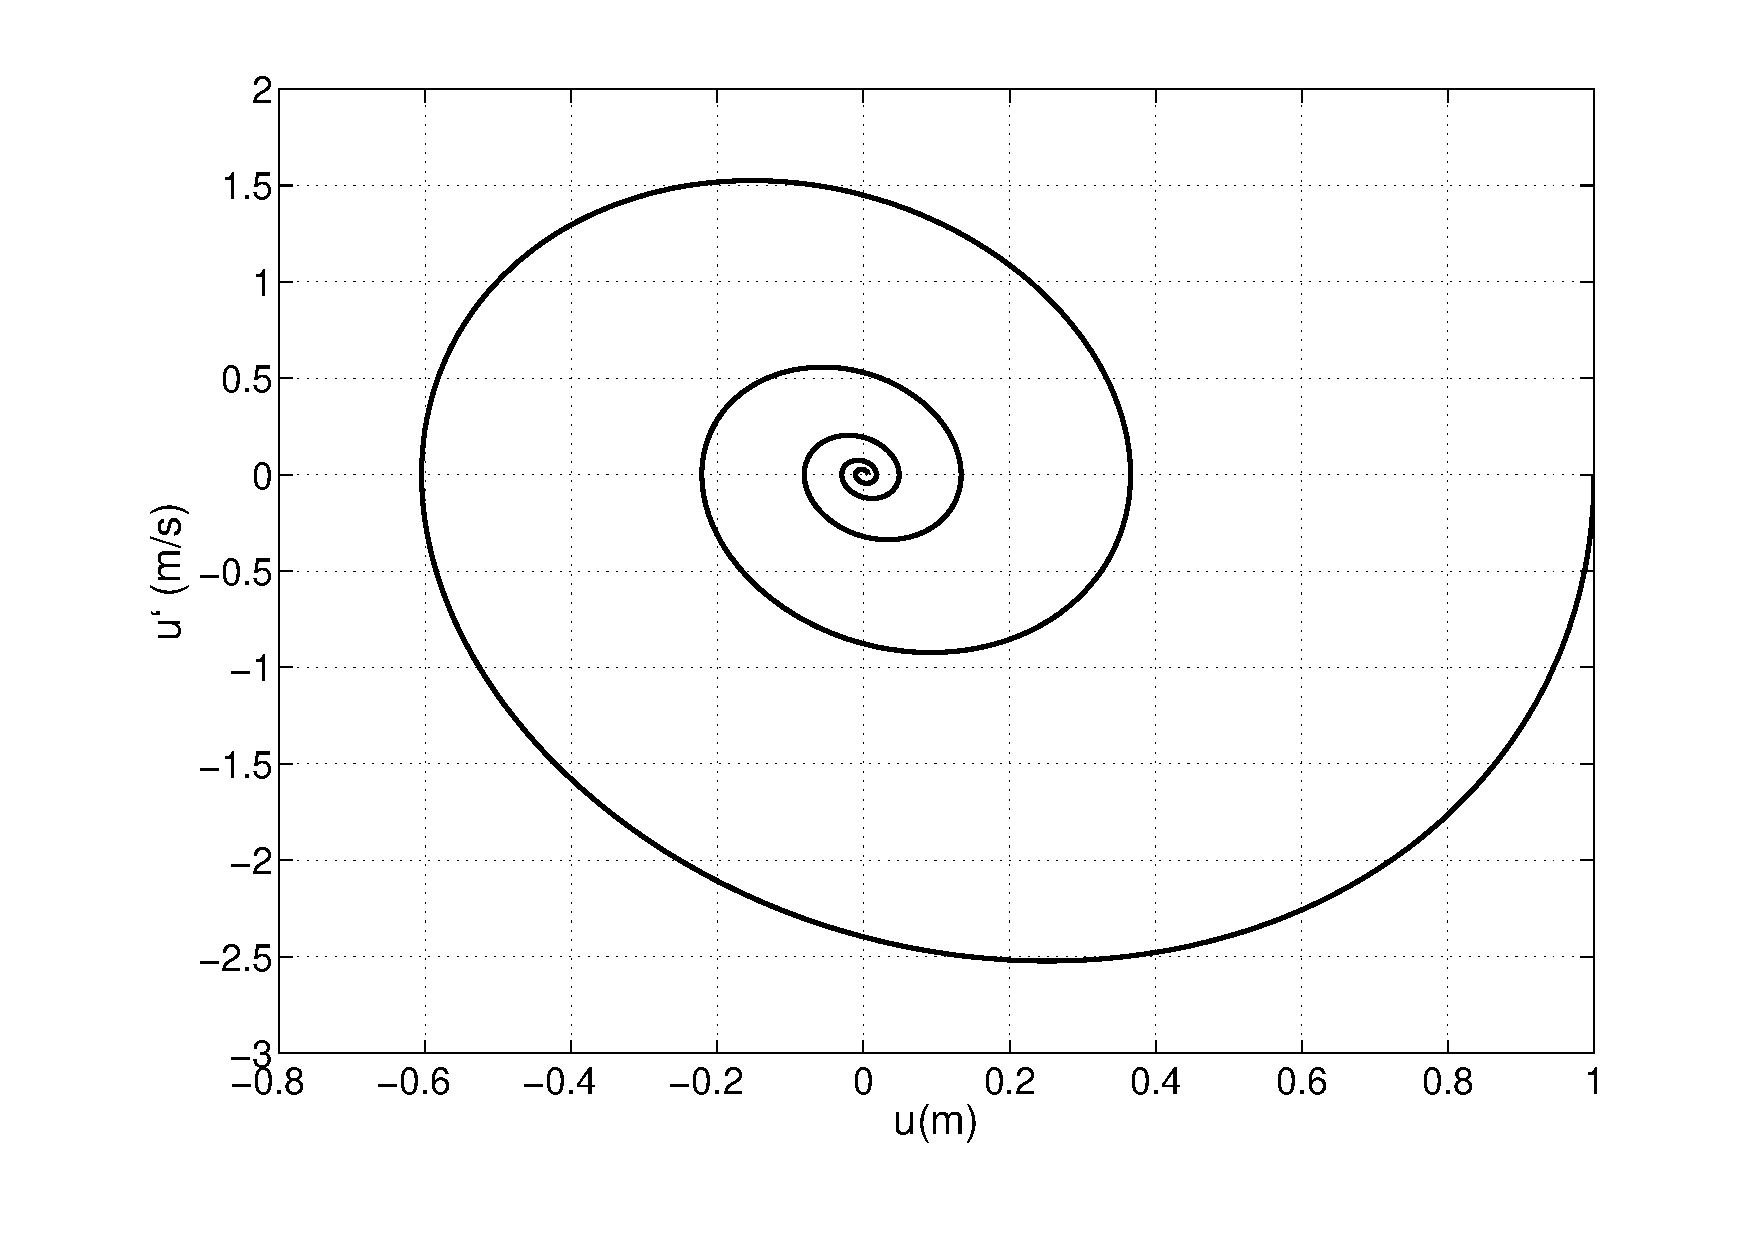
\includegraphics[scale=0.3, trim = 20mm 0mm 0mm 0mm, clip]{./Figures/2-CauchyProblem/D=1_uu.pdf}
\caption{Position ($u$) vs. velocity ($\dot{u}$) for the damped system.}
\end{figure}

\end{multicols}

This kind of easy examples are very useful for testing and validating the
software applications. Once again the results were successful, so the
functionality of the Cauchy module is assured. \\







